\documentclass[11pt]{beamer}
\usepackage[utf8]{inputenc}
\usepackage{lmodern}
%\usepackage{subfig}
\usepackage{caption}

\setbeamertemplate{navigation symbols}{}

\usetheme{Warsaw}
\usecolortheme[RGB={32,69,96}]{structure}
\beamersetuncovermixins{\opaqueness<1>{75}}{\opaqueness<2->{55}}
\addtobeamertemplate{footline}{\hfill\insertframenumber/\inserttotalframenumber\hspace{2em}\null}
%\beamertemplatetransparentcovered


\newcommand {\framedgraphic}[2] {
    \begin{frame}{#1}
        \begin{center}
            \includegraphics[width=\textwidth,height=0.8\textheight,keepaspectratio]{#2}
        \end{center}
    \end{frame}
}

\title{Génération Automatique de Texte}
\subtitle{Soutenance projet de programmation}
\author{B. Barthés \\ A. Boumera \\ B. Guiomar \\ C. Pennarun \\ A. Wintringer}
\date{Mardi 16 Avril 2013}

\begin{document} 
\begin{frame}
\titlepage
\end{frame}

\section*{Introduction}
\begin{frame}\frametitle{Introduction}
	\setbeamercovered{transparent}
\begin{itemize}
\uncover<1>{\item Génération Automatique de Texte}
\uncover<2>{\item Existant}
\uncover<3>{\item Objectifs du projet}
\end{itemize}

\end{frame}

\section{Déroulement du logiciel}

\subsection{Administrateur}

\subsubsection{Base de données}
\begin{frame}{Base de données}
\begin{block}{Création de projet}
\begin{center}
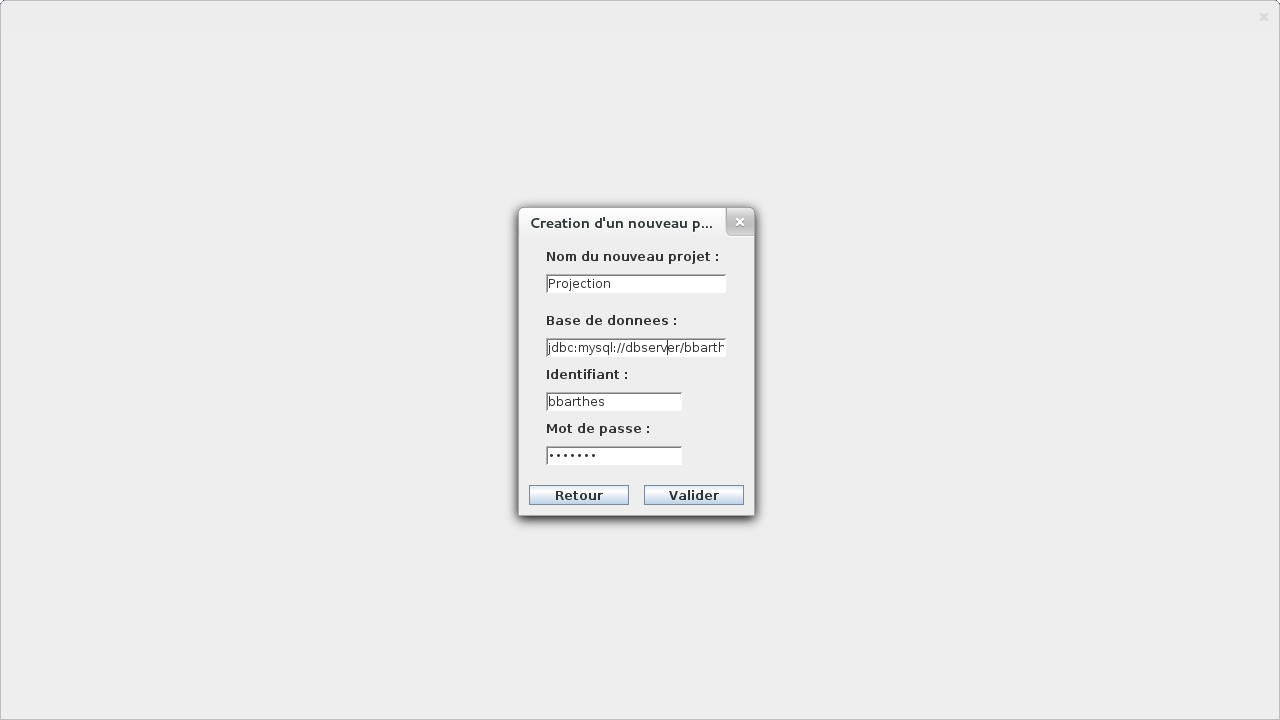
\includegraphics[scale=0.2]{db_connection.png}
\end{center}
\end{block}
\end{frame}

\begin{frame}{Base de données}
\begin{block}{Organisation de la base de données}
\begin{center}
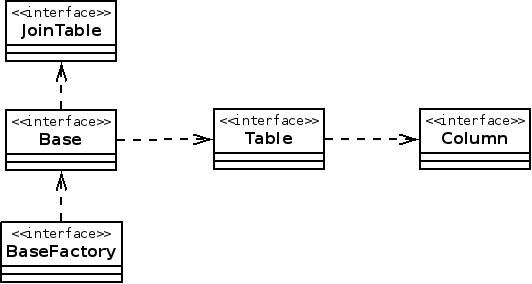
\includegraphics[scale=0.3]{db_presentation.png}
\end{center}
\end{block}
\end{frame}

\subsubsection{Base de données}
\begin{frame}{Base de données}
\begin{block}{Création de types}
\begin{center}
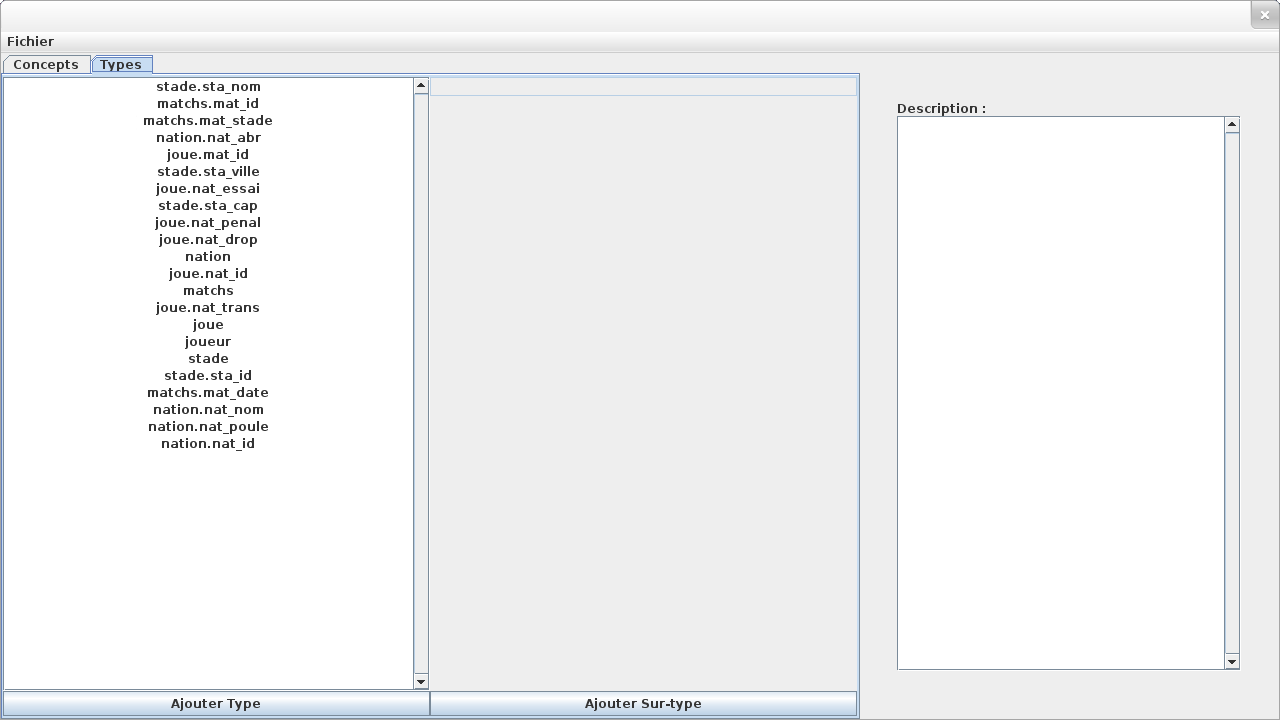
\includegraphics[scale=0.2]{creation_types.png}
\end{center}
\end{block}
\end{frame}


\subsubsection{Concepts et système de typage}
\begin{frame}{Concepts et système de typage}
\begin{columns}

\begin{column}{6cm}

\setbeamercovered{transparent}
\begin{itemize}[<+->]
\item Types
\\ \only<1>{Définis par un nom et un surtype}
\item Concepts
\\ \only<2>{Définis par un nom, un type et des types arguments}
\item Scénarios
\\ \only<3>{Liste de graphes de concepts}
\item Projet
\\ \only<4>{Défini par un nom, des scénarios, l'ensemble des types et des concepts et les informations de la base de données}
\end{itemize}

\end{column}

\begin{column}{6cm}
\only<1>{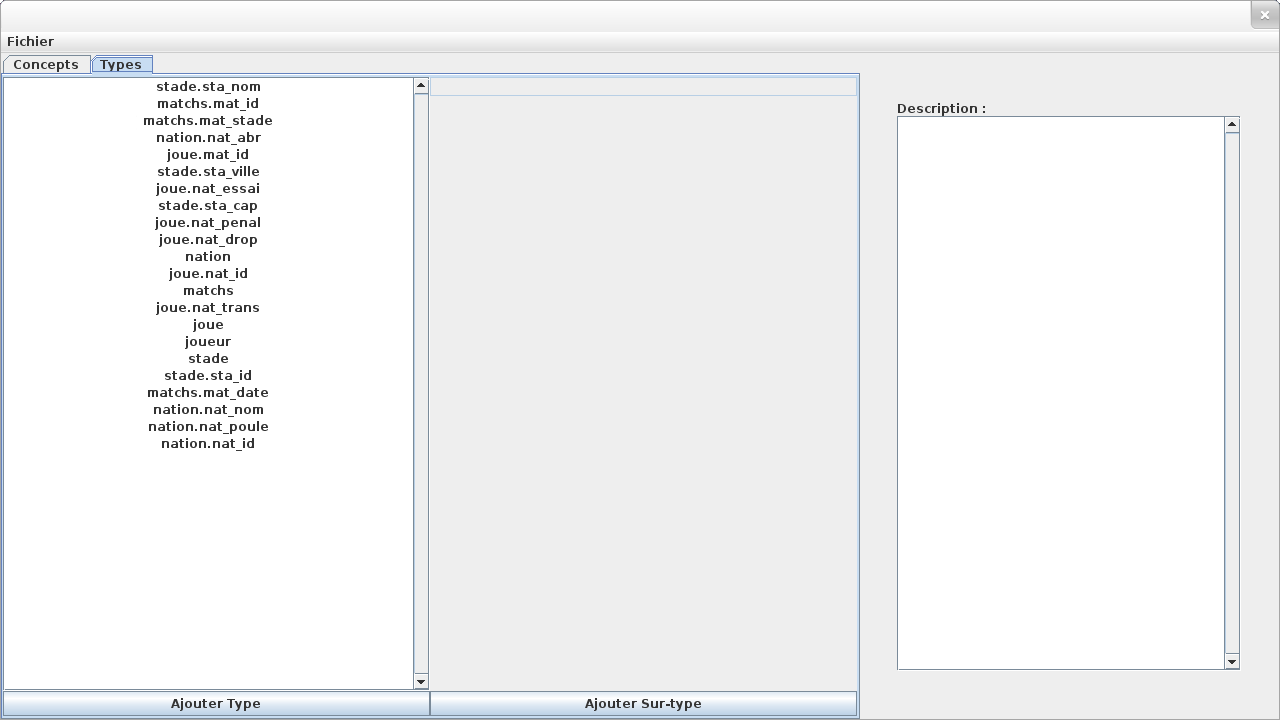
\includegraphics[scale=0.135]{creation_types.png}
\captionof{figure}{Fenêtre création de types}}

\only<2>{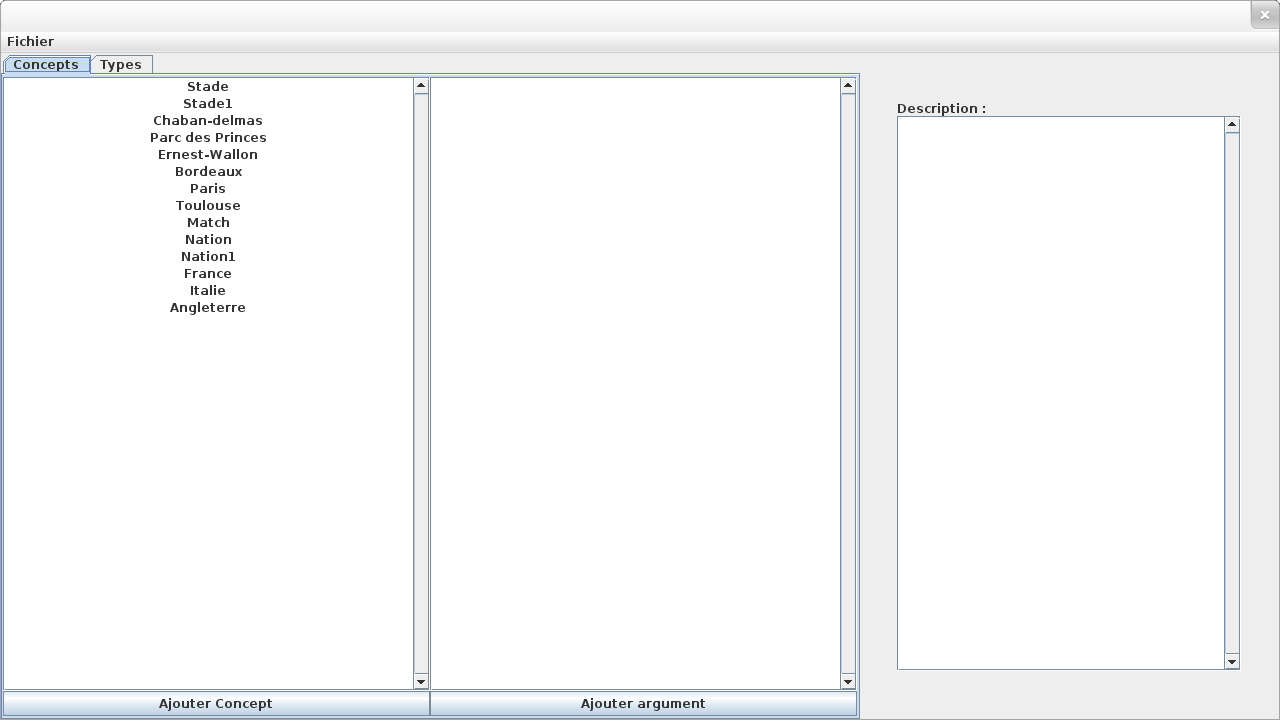
\includegraphics[scale=0.135]{creation_concepts.png}
\captionof{figure}{Fenêtre création de concepts}}

\only<3->{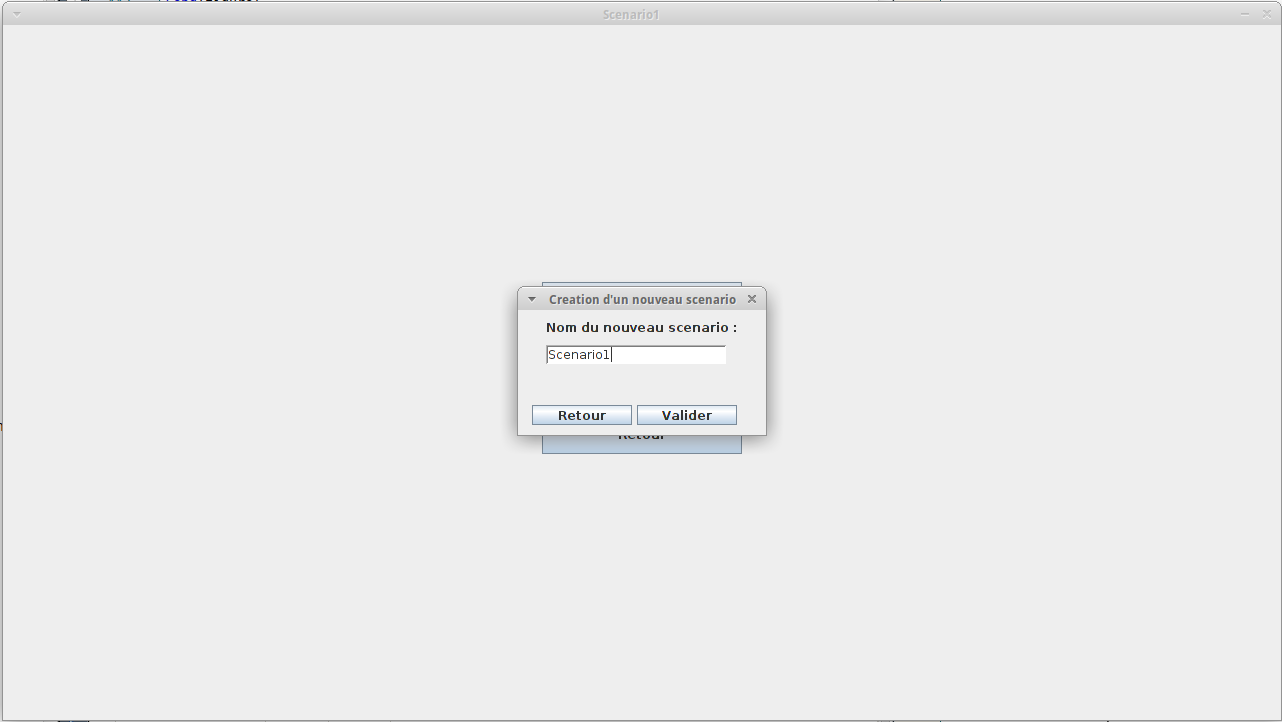
\includegraphics[scale=0.135]{creation_scenario.png}
\captionof{figure}[]{Fenêtre création de scénarios}}
\end{column}

\end{columns}
\end{frame}





\subsubsection{Sauvegarde}
\begin{frame}{Sauvegarde}
\setbeamercovered{transparent}
\begin{itemize}[<+->]
\item Enregistrement de l'objet Projet
\item Utilisation de la bibliothèque xstream pour l'enregistrement des fichiers en .xml
\end{itemize}
\end{frame}


\subsection{Utilisateur}

\subsubsection{Graphes conceptuels}

\begin{frame}{Graphes conceptuels}
\setbeamercovered{transparent}

\only<1-4>{
\uncover<1-4>{Point technique : rajout d'un noeud dans le graphe conceptuel}

\uncover<2-4>{\bigskip Problème : besoin d'une structure arborescente}
\uncover<3-4>{\\ MAIS plusieurs noeuds peuvent référencer le même Concept}

\uncover<4>{\bigskip Solution proposée : 
	\begin{itemize}
	\item utilisation d'un tag
	\item création d'une référence
	\end{itemize}
}
}

\only<5->{
\uncover<5->{Ajout d'un GraphNode child sur un GraphNode parent}
\begin{itemize} 
\uncover<6->{\item on vérifie la compatibilité de child et parent}
\uncover<7->{\item si le noeud child est tagué}
				\uncover<8->{\\ on en crée une copie, qui en contient une référence}
				\uncover<9->{\\ on signale que child possède une référence}
 \uncover<10->{\item sinon, on met un tag dessus et on l'ajoute}
\end{itemize}

\uncover<11->{\bigskip Remarque : pas besoin de regarder les "enfants" du noeud à rajouter}
}
\end{frame}


\subsubsection{Connexion à Syntox}
\begin{frame}{Connexion à Syntox}
\begin{block}{Fonctionnement souhaité}
\begin{center}
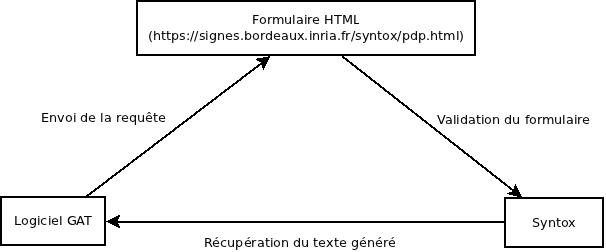
\includegraphics[scale=0.35]{syntox_connection.jpg}
\end{center}
Problème technique: \\ Le texte généré par Syntox n'était pas obtenu, l'action du formulaire ne semblait pas se déclencher. \\
\end{block}
\end{frame}

\begin{frame}{Connexion à Syntox}
\setbeamercovered{transparent}
\uncover<1->{Génération de la requête par le graphe conceptuel}

\uncover<2->{\bigskip
Rappel des besoins:}
\begin{itemize}
\uncover<3->{\item communiquer avec Syntox,}
\uncover<4->{\item soumettre la requête,}
\uncover<5->{\item récupérer et afficher le résultat.}
\end{itemize}
\uncover<6->{\bigskip Idée: déclencher de manière sûre l'action du formulaire.}
\end{frame}

\begin{frame}{Connexion à Syntox}
\begin{block}{Solution élaborée - Création de la page "pdp.html" en local}

\begin{center}
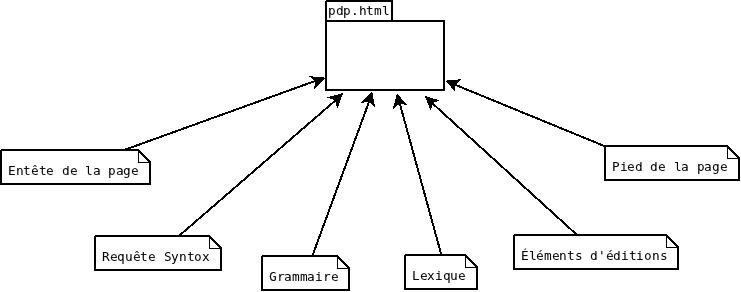
\includegraphics[scale=0.3]{syntox_connection2.png}
\end{center}
Transformation en fichier des champs masqués (Grammaire, lexique et éléments d'édition)
\\ Lancement automatique depuis le navigateur par défaut
\end{block}
\end{frame}

\begin{frame}{Connexion à Syntox}
\begin{block}{Avantages}
\begin{itemize}
\item page en local, pas besoin d'avoir Internet pour la créer,
\item la requête peut être modifiée avant d'être envoyée à Syntox,
\item les fichiers de grammaire, lexique et éléments d'édition peuvent être édités.
\end{itemize}
\end{block}
\begin{block}{Inconvénients}
\begin{itemize}
\item l'utilisateur doit lui même appuyer sur le bouton pour générer l'action du formulaire,
\item la mise à jour des fichiers doit se faire manuellement,
\item un navigateur Internet désigné par défaut doit être présent.
\end{itemize}
\end{block}
\end{frame}

\section{Architecture}
\begin{frame}{Architecture}
\begin{block}{Diagramme de packages}
\begin{center}
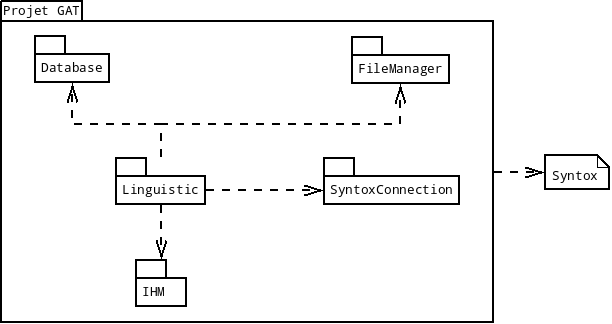
\includegraphics[scale=0.4]{DiagPackages.png}
\end{center}
\end{block}
\end{frame}

\section{Tests}
\begin{frame}{Tests}

\uncover<1->{Effectués sur les packages \texttt{linguistic} et \texttt{core}}

\setbeamercovered{transparent}

\uncover<1->{\bigskip Package \texttt{linguistic}}
\begin{itemize}
\uncover<2->{\item Concepts,}
\uncover<3->{\item Types,}
\uncover<4->{\item Graphe conceptuel.}
\end{itemize}

\uncover<5->{Package \texttt{core}}
\begin{itemize}
\uncover<6->{\item cryptage du mot de passe,}
\uncover<7->{\item ajout/suppression de scénarios à un projet.}
\end{itemize}
\end{frame}


\section{Conclusion et perspectives}
\begin{frame}{Conclusion et perspectives}
\setbeamercovered{transparent}
\begin{itemize}[<+->]
\item Interface graphique
\item Linguistique
\item Base de données
\item Connexion Syntox
\end{itemize}
\end{frame}


\end{document}
 
